% Terceira lista de exerc�cios de Sistemas e Sinais
% Preparado para MiKTeX 2.9. Gerar arquivo PDF com pdflatex.
\documentclass[12pt,fleqn]{amsart}
\usepackage{enumitem}
\usepackage{xstring}
\usepackage{graphicx}
\usepackage[a4paper]{geometry}
\usepackage[portuguese,brazilian]{babel}
\usepackage[ansinew]{inputenc}
\usepackage[T1]{fontenc}
\usepackage{comment}
% Fontes
\usepackage{textgreek}
\usepackage{yfonts}
\usepackage{microtype}
\usepackage{calligra}
\usepackage{lmodern}
\usepackage{bookman}
\usepackage[scaled]{helvet}
\usepackage[usenames,dvipsnames,svgnames,table]{xcolor}
\usepackage[hyphens]{url}
\usepackage{hyperref}
\usepackage{fmtcount}
% Formata��o
\usepackage{sidecap}
\usepackage{float}
\usepackage{listings}
\usepackage{matlab-prettifier}
% S�mbolos matem�ticos
\usepackage{amsmath}
\usepackage{amssymb}
\usepackage{wasysym}
\usepackage{mathtools}
\usepackage{bbm}
\usepackage{mbboard}
\usepackage{steinmetz}
% Desenhos
\usepackage{tikz}
\usepackage{circuitikz}


\title{Sistemas e Sinais - Exerc�cio III}
\date{}
\author{S�rgio Cordeiro}


\newenvironment{pergunta}{
	\par
	\trivlist
	\fontfamily{phv}
	\selectfont
	\item\arabic{prob_num}. 
	}{
	\endtrivlist
	}

\newenvironment{resposta}{
	\trivlist
    \vspace{3pt}
	\fontfamily{pbk}
	\selectfont
	\item
	}{
	\vspace{3pt}
	\noindent\makebox[\linewidth]{\rule{\paperwidth}{1pt}}
	\endtrivlist
	\stepcounter{prob_num}
	}

\newenvironment{listae}[1][]{
  \IfStrEqCase{#1}{
    {1}{\setenumerate[0]{label=\arabic*.}}
    {2}{\setenumerate[0]{label=\alph*)}}
    {3}{\setenumerate[0]{label=\roman*.}}
	{}{\setenumerate[0]{label=\arabic*)}}}
	\vspace{-5mm}
	\begin{enumerate}}{
	\end{enumerate}	
	\vspace{-5mm}}

\newenvironment{listaef}[1][]{
  \IfStrEqCase{#1}{
    {1}{\setenumerate[0]{label=\arabic*.}}
    {2}{\setenumerate[0]{label=\alph*)}}
    {3}{\setenumerate[0]{label=\roman*.}}
	{}{\setenumerate[0]{label=\arabic*)}}}
	\vspace{-5mm}
	\begin{enumerate}}{
	\end{enumerate}}

\DeclareMathAlphabet{\mathpzc}{OT1}{pzc}{m}{it}

\DeclareMathOperator{\La}{\mathcal{L}}					% Transformada de Laplace
\DeclareMathOperator{\De}{\boldsymbol{\delta}}			% Fun��o impulso
\DeclareMathOperator{\dDe}{\boldsymbol{\dot{\delta}}}	% Derivada da fun��o impulso
\newcommand{\dt}[1]{\frac{d {#1}}{dt}}					% derivada temporal
\newcommand{\ddt}[1]{\frac{d^2 {#1}}{dt^2}}				% derivada segunda temporal
\newcommand{\dtau}[1]{\frac{d {#1}}{d \tau}}			% derivada temporal
\newcommand{\ddtau}[1]{\frac{d^2 {#1}}{d \tau^2}}		% derivada segunda temporal


% Linhas divis�rias
\newcommand{\hhhlin}{\noindent\hfil\rule{0.25\textwidth}{.2pt}\hfil\newline}
\newcommand{\hhlin}{\noindent\hfil\rule{0.5\textwidth}{.4pt}\hfil\newline}
\newcommand{\hlin}{\noindent\hfil\rule{\textwidth}{.8pt}\hfil\newline}

% Cita��es
\newcommand{\newbibit}[6]{\bibitem[#1]{#2}#3, {\bf #4}. Dispon�vel em \url{#5}, acesso em #6.}
\newcommand{\newbibpp}[5]{\bibitem[#1]{#2}#3, {\bf #4}, \emph{in} #5.}
\newcommand{\newbibbk}[5]{\bibitem[#1]{#2}#3, {\bf #4}, #5.}
\newcommand{\newbibip}[6]{\bibitem[#1]{#2}#3, {\bf #4}, \emph{in} #5, dispon�vel em \url{#6}.}
\newcommand{\newbiboc}[4]{\bibitem[#1]{#2}#3, \textit{op. cit.}, #4.}
\newcommand{\newbibsi}[7]{\bibitem[#1]{#2}#3, {\bf #4} : {#5}. Dispon�vel em \url{#6}, acesso em #7.}

\newenvironment{iquote}{\begin{quote}\itshape}{\end{quote}}

% Perguntas
\newcommand{\perguntaa}{Pesquisar a origem do termo "equa��o de diferen�as". \\
}
\newcommand{\perguntab}{Gerar no MATLAB a sequ�ncia $ f[n] = \cos (\Omega n) $ com:
\begin{align}
	\Omega & = 0.2 \pi \\
	\Omega & = 0.3 \pi \\
	\Omega & = 0.8
\end{align}
e $ 0 \le n \le 100 $ e plotar o resultado.
}
\newcommand{\perguntac}{Dada a equa��o de diferen�as abaixo, que define um sistema:
\begin{align}
	y[n+2] + 6 y[n+1] + 25 y[n] = 3 e[k]
\end{align}
\begin{listae}[1]
	\item Encontrar a resposta do sistema ao impulso.
	\item Calcular a resposta ao impulso por meio da convolu��o.
\end{listae}
}


\begin{document}
\setlength{\parskip}{1em}
\setlength{\jot}{10pt}
\setlength{\parindent}{0pt}

\maketitle

\newcounter{prob_num}
\setcounter{prob_num}{1}


\iffalse
\begin{pergunta}
\perguntaa{}
\end{pergunta}
\begin{resposta}
\end{resposta}
\fi

\begin{pergunta}
\perguntab{}
\end{pergunta}
\begin{resposta}
Os gr�ficos s�o os seguintes:
\begin{figure}[H]
	\centering
	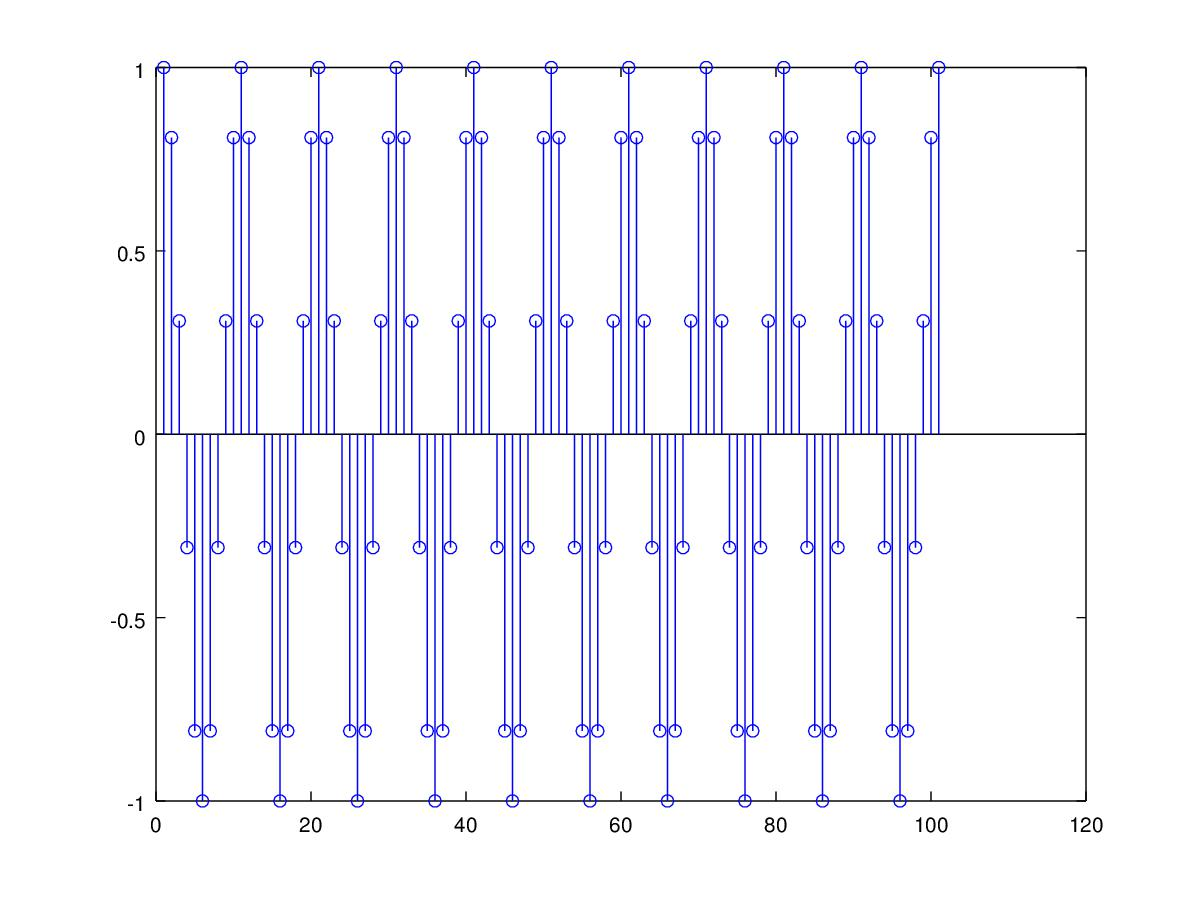
\includegraphics[width=0.7\textwidth]{trab28figb1.jpg} \\
	$ \Omega = 0.2 \pi $ \\
\end{figure}%
\begin{figure}[H]
	\centering
	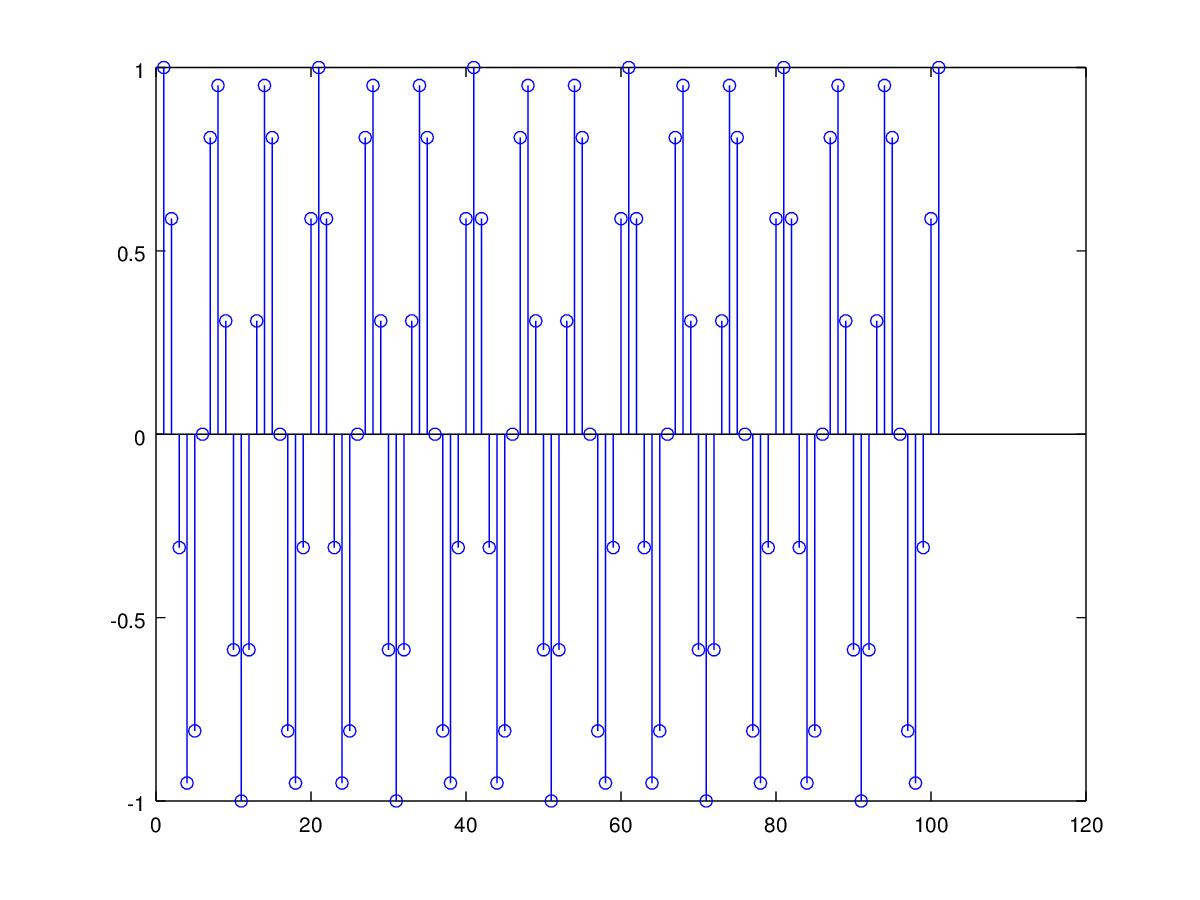
\includegraphics[width=0.7\textwidth]{trab28figb2.jpg} \\
	$ \Omega = 0.3 \pi $ \\
\end{figure}%
\begin{figure}[H]
	\centering
	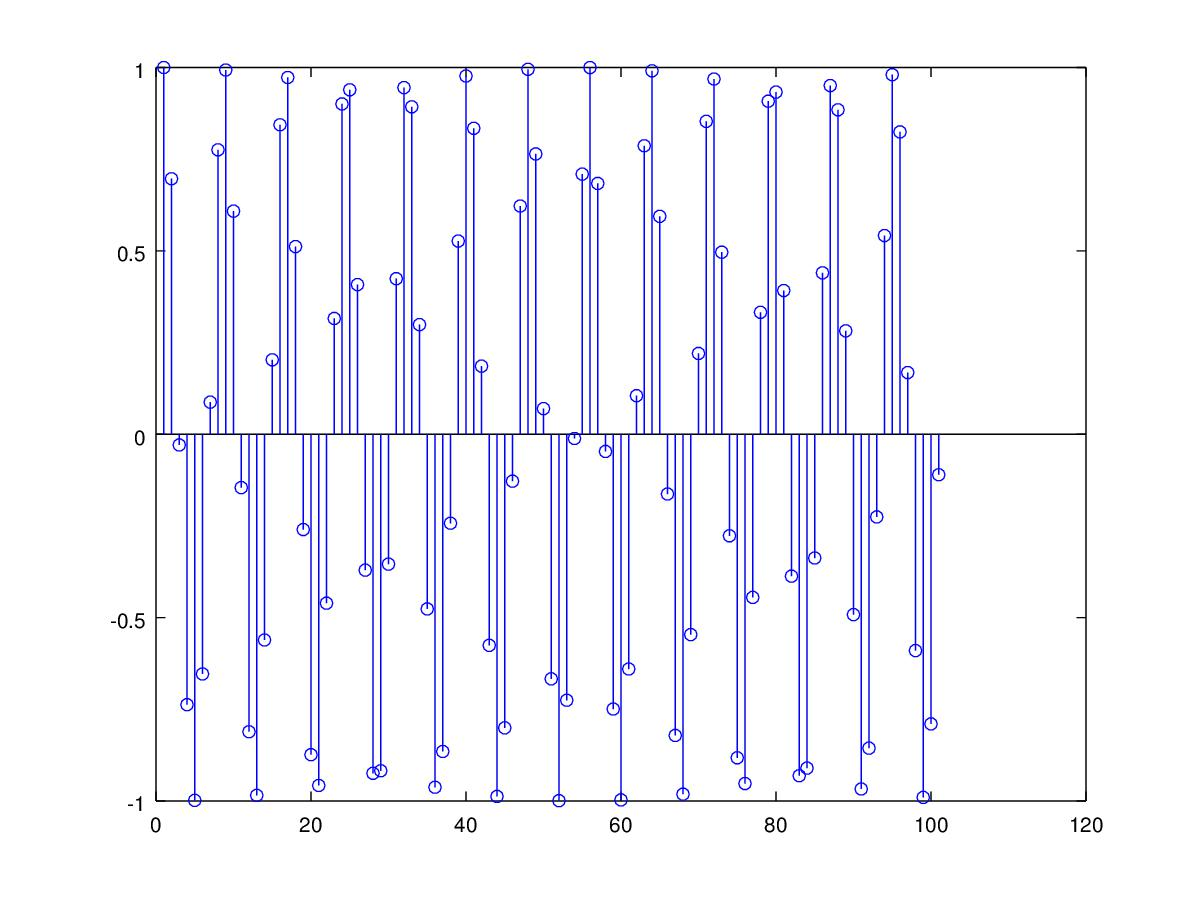
\includegraphics[width=0.7\textwidth]{trab28figb3.jpg} \\
	$ \Omega = 0.8 $ \\
\end{figure}%
\end{resposta}

\clearpage

\begin{pergunta}
\perguntac{}
\end{pergunta}
\begin{resposta}
A equa��o caracter�stica do sistema �:
\begin{align*}
	\gamma^2 + 6 \gamma + 25 = 0 \qquad \implies \gamma & = \frac{-6 \pm \sqrt{5^2 - 4.1.25}}{2} \\
	& = - 3 \pm \jmath 4 \\
	& = 5 \phase{\pm 2.21} \\
\end{align*}
A resposta natural, que tamb�m � a resposta ao impulso, � ent�o:
\begin{align*}
	h[n] = \mathrm{A} \gamma_1^n + \mathrm{B} \gamma_2^n \qquad \Aboxed{\gamma_1 = 5 \phase {2.21}, \; \gamma_2 = 5 \phase{-2.21}} \\
\end{align*}
Para as condi��es iniciais $ y[0] = 0, \; y[1] = 1 $, teremos: \\
\begin{align*}
	\mathrm{A} + \mathrm{B} = 0 \qquad & \implies \mathrm{A} = - \mathrm{B} \\
	\mathrm{A} \gamma_1 + \mathrm{B} \gamma_2 = 3 \qquad & \implies \mathrm{A} \gamma_1 - \mathrm{A} \gamma_2 = 3
\end{align*}
\begin{align*}
	\qquad \wasytherefore \; \mathrm{A} & = \frac{3}{\gamma_1 - \gamma_2} \\
	& = \frac{3}{- 3 + \jmath 4 + 3 + \jmath 4} \\
	& = \frac{3}{\jmath 8} \\
	\mathrm{B} & = - \mathrm{A} \\
	& = - \frac{3}{\jmath 8}
\end{align*}
Assim:
\begin{align*}
	h[n] & = \frac{3}{\jmath 8} \; \gamma_1^n - \frac{3}{\jmath 8} \; \gamma_2^n \\
	& = \frac{3}{\jmath 8} (5^n \phase{2.21 n} - 5^n \phase {-2.21 n}) \\
	& = \frac{3 \times 5^n}{\jmath 8} \left( \frac{}{} \cos(2.21 n) + \jmath \sin(2.21 n) - \cos{-2.21 n} - \jmath \sin(-2.21 n) \right) \\
	& = - \frac{3 \times 5^n}{4} \sin(2.21 n)
\end{align*}
O sistema � inst�vel, e a resposta ao impulso diverge rapidamente. 
\begin{figure}[H]
	\centering
	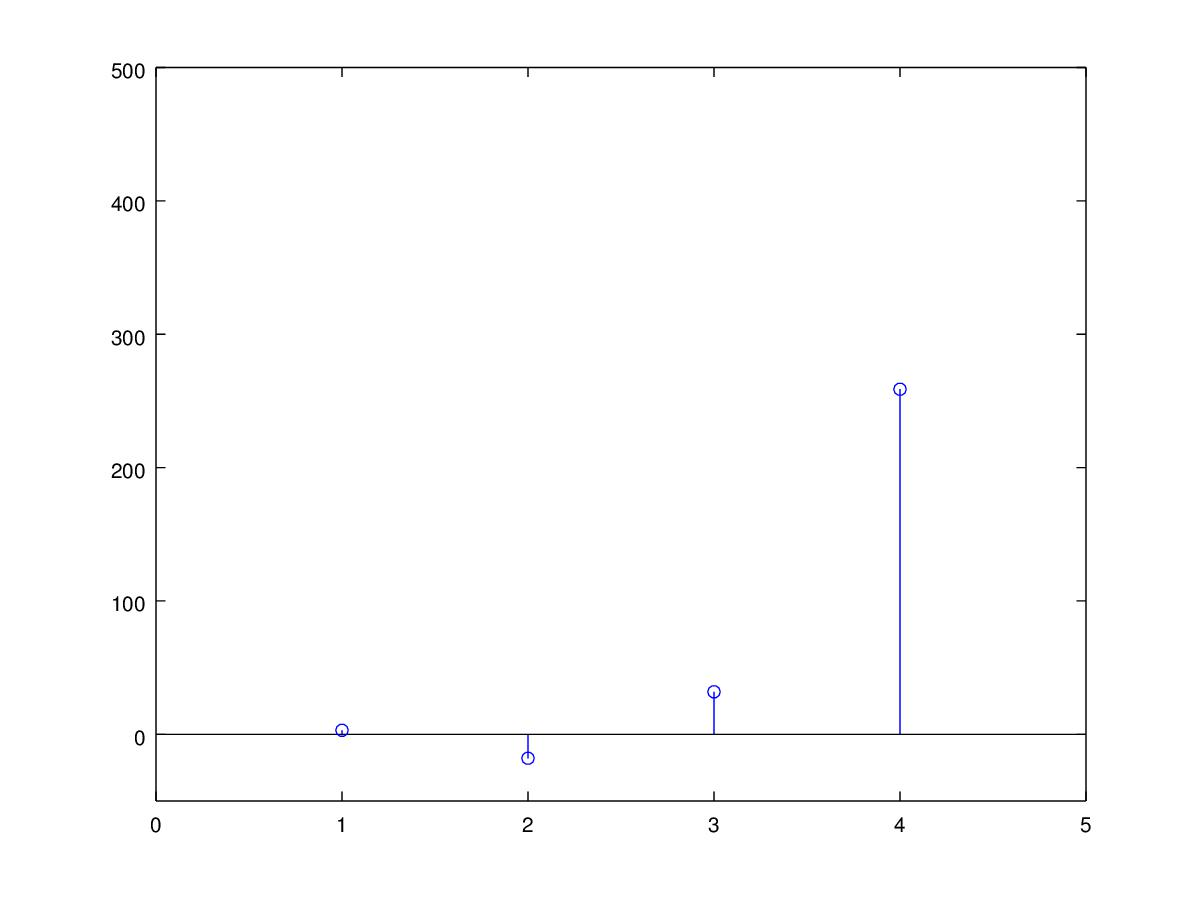
\includegraphics[width=0.7\textwidth]{trab28figc1.jpg} \\
	$ h[n] $ \\
\end{figure}%
A resposta a outro sinal $ e(t) $ pode ser obtida por convolu��o: $ y[n] = h[n] * e[n] $. Por exemplo, se $ e[n] $ � um degrau unit�rio ($ u[n] = {1, 1, 1...} $): \\
\begin{figure}[H]
	\centering
	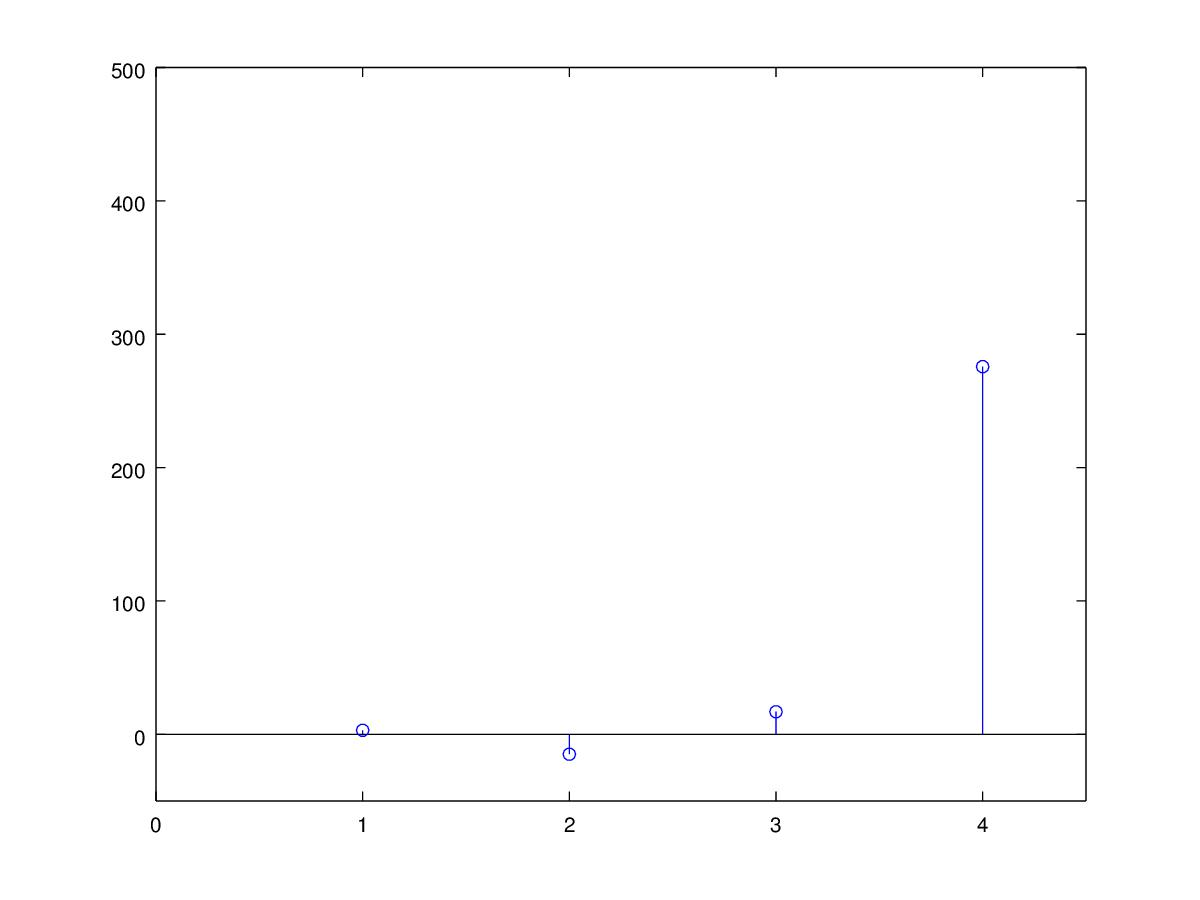
\includegraphics[width=0.7\textwidth]{trab28figc2.jpg} \\
	$ y[n] = h[n] * u[n] $ \\
\end{figure}%
\end{resposta}

\clearpage

Gr�ficos produzidos com \textbf{Octave} 4.0.0: \\
\url{https://www.gnu.org/software/octave/} \\
Texto formatado com \textbf{pdflatex} em ambiente \textbf{MiKTeX} 2.9: \\
\url{http://miktex.org/download/} \\ \\
\end{document}
